\chapter{Implementation}
\label{chap:implem}
\section {Development environment}
\section {InproTK Toolkit}
\subsection {Overview}
\subsection {IU Modules and Data Processing}
\begin{figure}[htbp]
  \centering
    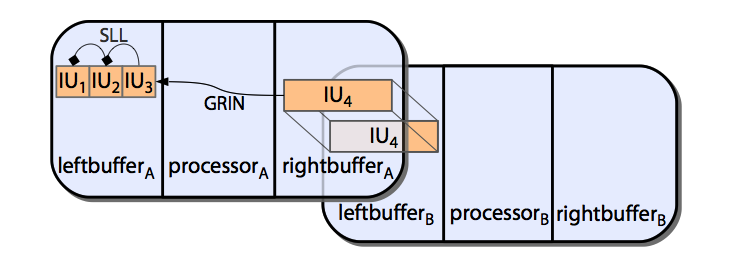
\includegraphics[width=1.0\textwidth]{images/iuandbuffer.png}
 \caption{ Incremental Units (IUs) and their intercommunication via left-right
 buffers}
  \label{fig:Bild1}
\end {figure}
\subsection {GoogleASR Module}
  \begin{figure}[htbp]
  \centering
   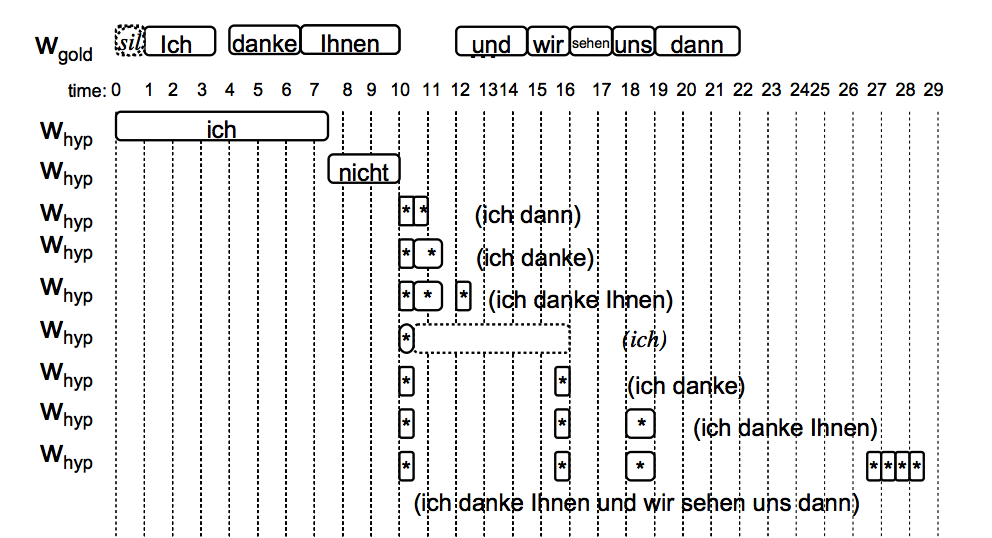
\includegraphics[width=0.9\textwidth]{images/google_output.png}
  \caption{Incremental output of Google ASR with existing timing}
  \label{fig:Bild1}
\end{figure}

\subsection {SphinxASR Module}

\section {Forced-alignment in InproTK}
\section {Architecture of the Implemented combined Google-Sphinx Recognizer}
\begin{figure}[htbp]
  \centering
    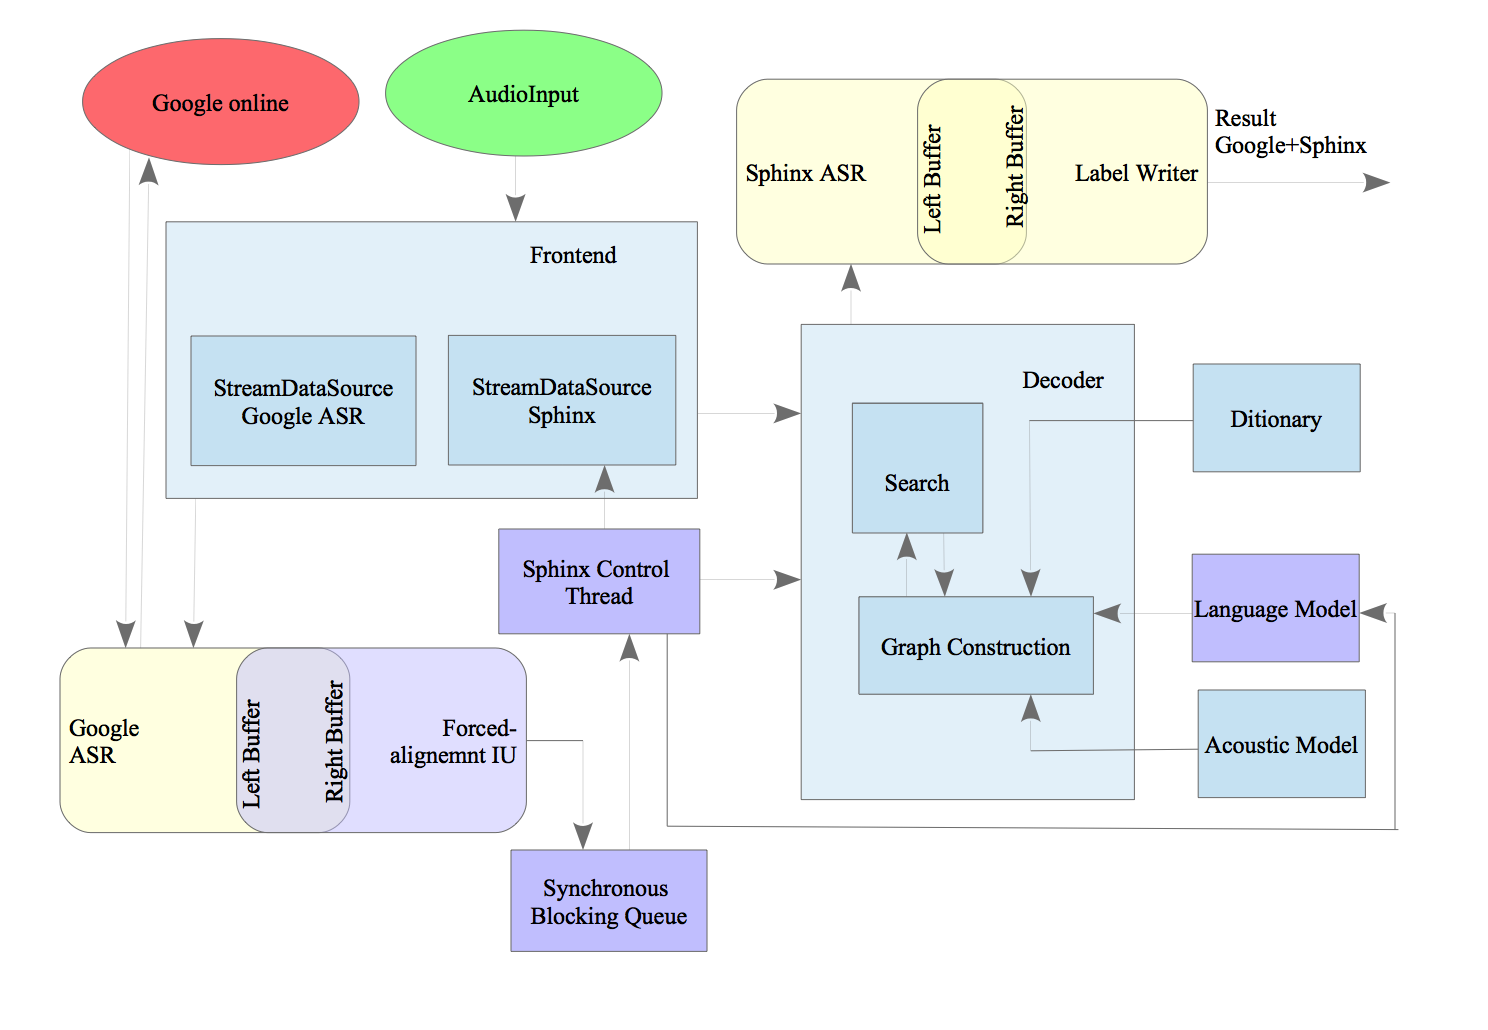
\includegraphics[width=0.8\textwidth]{images/architecture.png}
 \caption{Implementation Overview}
 
  \label{fig:Bild1}
\end {figure}
\section {Forced-alignment of Google Incremental Results with Google-Sphinx
Recognizer}
\section {Search Module of Google-Sphinx Recognizer}
\subsection {Decoder configuration}
\subsection {Search Modification}